\subsection{Modelo de iOS}
\begin{frame}
 \begin{center}
  \LARGE Modelo de iOS
 \end{center}
\end{frame}
\begin{frame}
 \frametitle{Modelo de iOS}
 \begin{figure}[H]
  \begin{subfigure}{0.7\linewidth}
   \begin{itemize}
    \item iOS es un sistema operativo para dispositivos móviles de la multinacional Apple Inc. diseñado para ser
seguro. \pause
    \item Cada dispositivo combina hardware, software y servicios, diseñados para trabajar conjuntamente para proveer seguridad y al mismo tiempo, que sea transparente para el usuario. \pause
    \item Las principales características de seguridad, como el cifrado del dispositivo, no son configurables y vienen habilitadas por defecto.\pause
    \item La seguridad se extiende más allá del dispositivo, incluido todo lo que hacen los usuarios localmente, en redes y con servicios clave de Internet, generando un ecosistema seguro.
   \end{itemize}
  \end{subfigure}
  \begin{subfigure}{0.23\linewidth}\pause
    \centering
    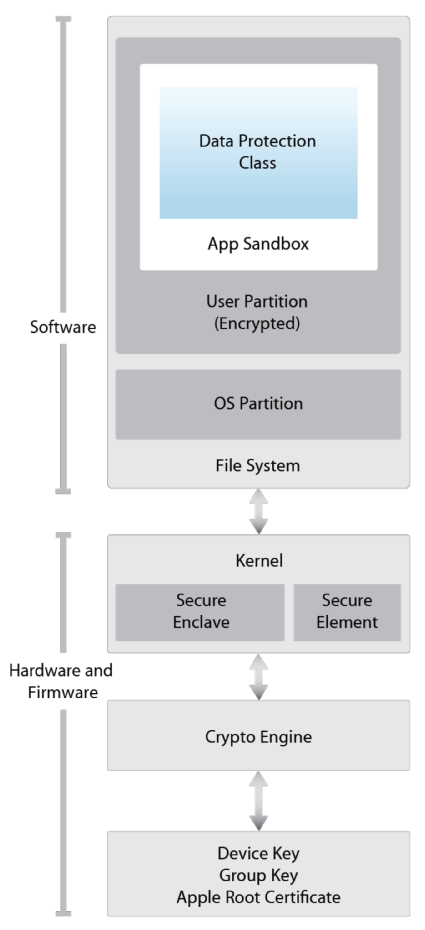
\includegraphics[width=\linewidth]{ios_security_architecture}
    \caption{Modelo de seguridad de iOS.}
  \end{subfigure}
\end{figure}
\end{frame}
\begin{frame}
 \frametitle{Modelo de iOS}
 \begin{itemize}
  \item Cada aplicación instalada por el usuario se ejecuta en un \emph{entorno aislado}\footnote{Traducción propuesta para el término \textit{sandbox}.}.\pause
  \item Como consecuencia de esto, tiene denegado el acceso a los archivos guardados por otra aplicación y no puede realizar cambios en el dispositivo. \pause Si una aplicación requiere acceder a información que no es suya, lo puede hacer únicamente usando servicios de iOS.\pause
  \item iOS ayuda a evitar que las aplicaciones accedan a la información personal de un usuario sin permiso.\pause
  \item Para acceder a ciertos recursos necesita autorización explícita del usuario.\pause
  \item Las aplicaciones pueden solicitar un permiso solamente mientras se esté ejecutando. \pause A su vez, los usuarios pueden optar por no permitir este acceso, y pueden cambiar su elección en cualquier momento.
 \end{itemize}
\end{frame}
\begin{frame}
 \frametitle{Modelo de iOS}
 \begin{itemize}
  \item De querer otorgar o revocar algún permiso, el usuario debe ir a la configuración de privacidad (\texttt{Ajustes/Privacidad}).
 \end{itemize}
 \begin{figure}[hbtp]
    \centering
    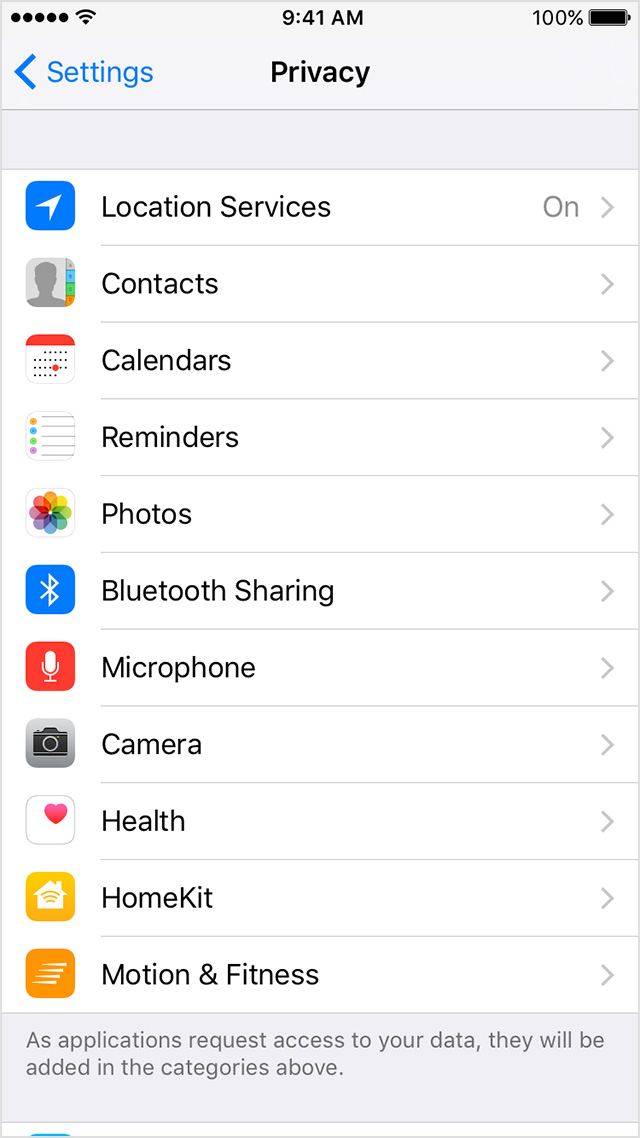
\includegraphics[width=.25\linewidth]{settings-privacy}
    \caption{Control de privacidad de iOS 9.}
 \end{figure}
\end{frame}
